\documentclass[../thesis.tex]{subfiles}
\begin{document}
\chapter{Commercial Scope}


Organic electronics is an exciting technology that is rising in commercial popularity.\supercite{Kenning2017,Soneira2016,Soneira2017}
These devices exhibit a number of unique features that allow them to compete with traditional semiconductors, as well as occupy new technological space.
This has been leveraged in various technologies, including organic light-emitting devices (OLEDs), photovoltaics (OPVs), and field effect transistors (OFETs).\supercite{Dimitrakopoulos2002,P.Gaj2016,Peumans2003}
This chapter seeks to provide an overview of applications as well as outline the focus of this work.

\section{Organic Devices}

Many of the advantages of organic electronics exist across all devices.  
Since the molecules are semiconductors on their own and do not rely on crystallinity, organic electronics are Van Der Waals bonded and are applied as thin films so do not have to be planar and rigid.  
This allows compatibility with flexible substrates and has been demonstrated for a variety of flexible devices.\supercite{Park2011,Gu1997,Sugimoto2004}
Additionally, curved and form fitting devices already exist in commercial devices.\supercite{Cok2005,Han2014a}

Compatibility with flexible substrates and a variety of processing techniques also unlocks the possibility of roll-to-roll and web processing.\supercite{Sondergaard2013}
Currently, commercial organic electronics primarily utilize vacuum deposition and batch processing, leading to relatively high cost devices.\supercite{Hung2015,Tsujimura2012}
As manufacturing techniques transition to roll-to-roll methods, mass production will offer a great reduction in device cost and will significantly alter the economics of organic electronics.
Roll-to-roll compatible device manufacturing methods so far have not demonstrated the highest efficiency devices and requires further development, though some commercial products do use solution processing.\supercite{Fahlteich,Manners2016,Mertens2016}

Most organic electronics utilize thin films, with total device thicknesses less than 500 nm of active material.  
This makes them compatible with extremely thin form factor devices, which are essential for mobile devices and small form factor electronics.
As wearable electronics become increasingly important, organic electronics being thin and flexible offer an obvious solution.

Organic molecules consist primarily of earth abundant materials such as carbon and nitrogen.  
Molecular structures of these materials can be easily modified, allowing for easy tuning of the molecular properties, such as emission and absorption.


\subsection{Organic Light-Emitting Devices (OLEDs)}

\begin{wrapfigure}{r}{.45\textwidth}
\centering
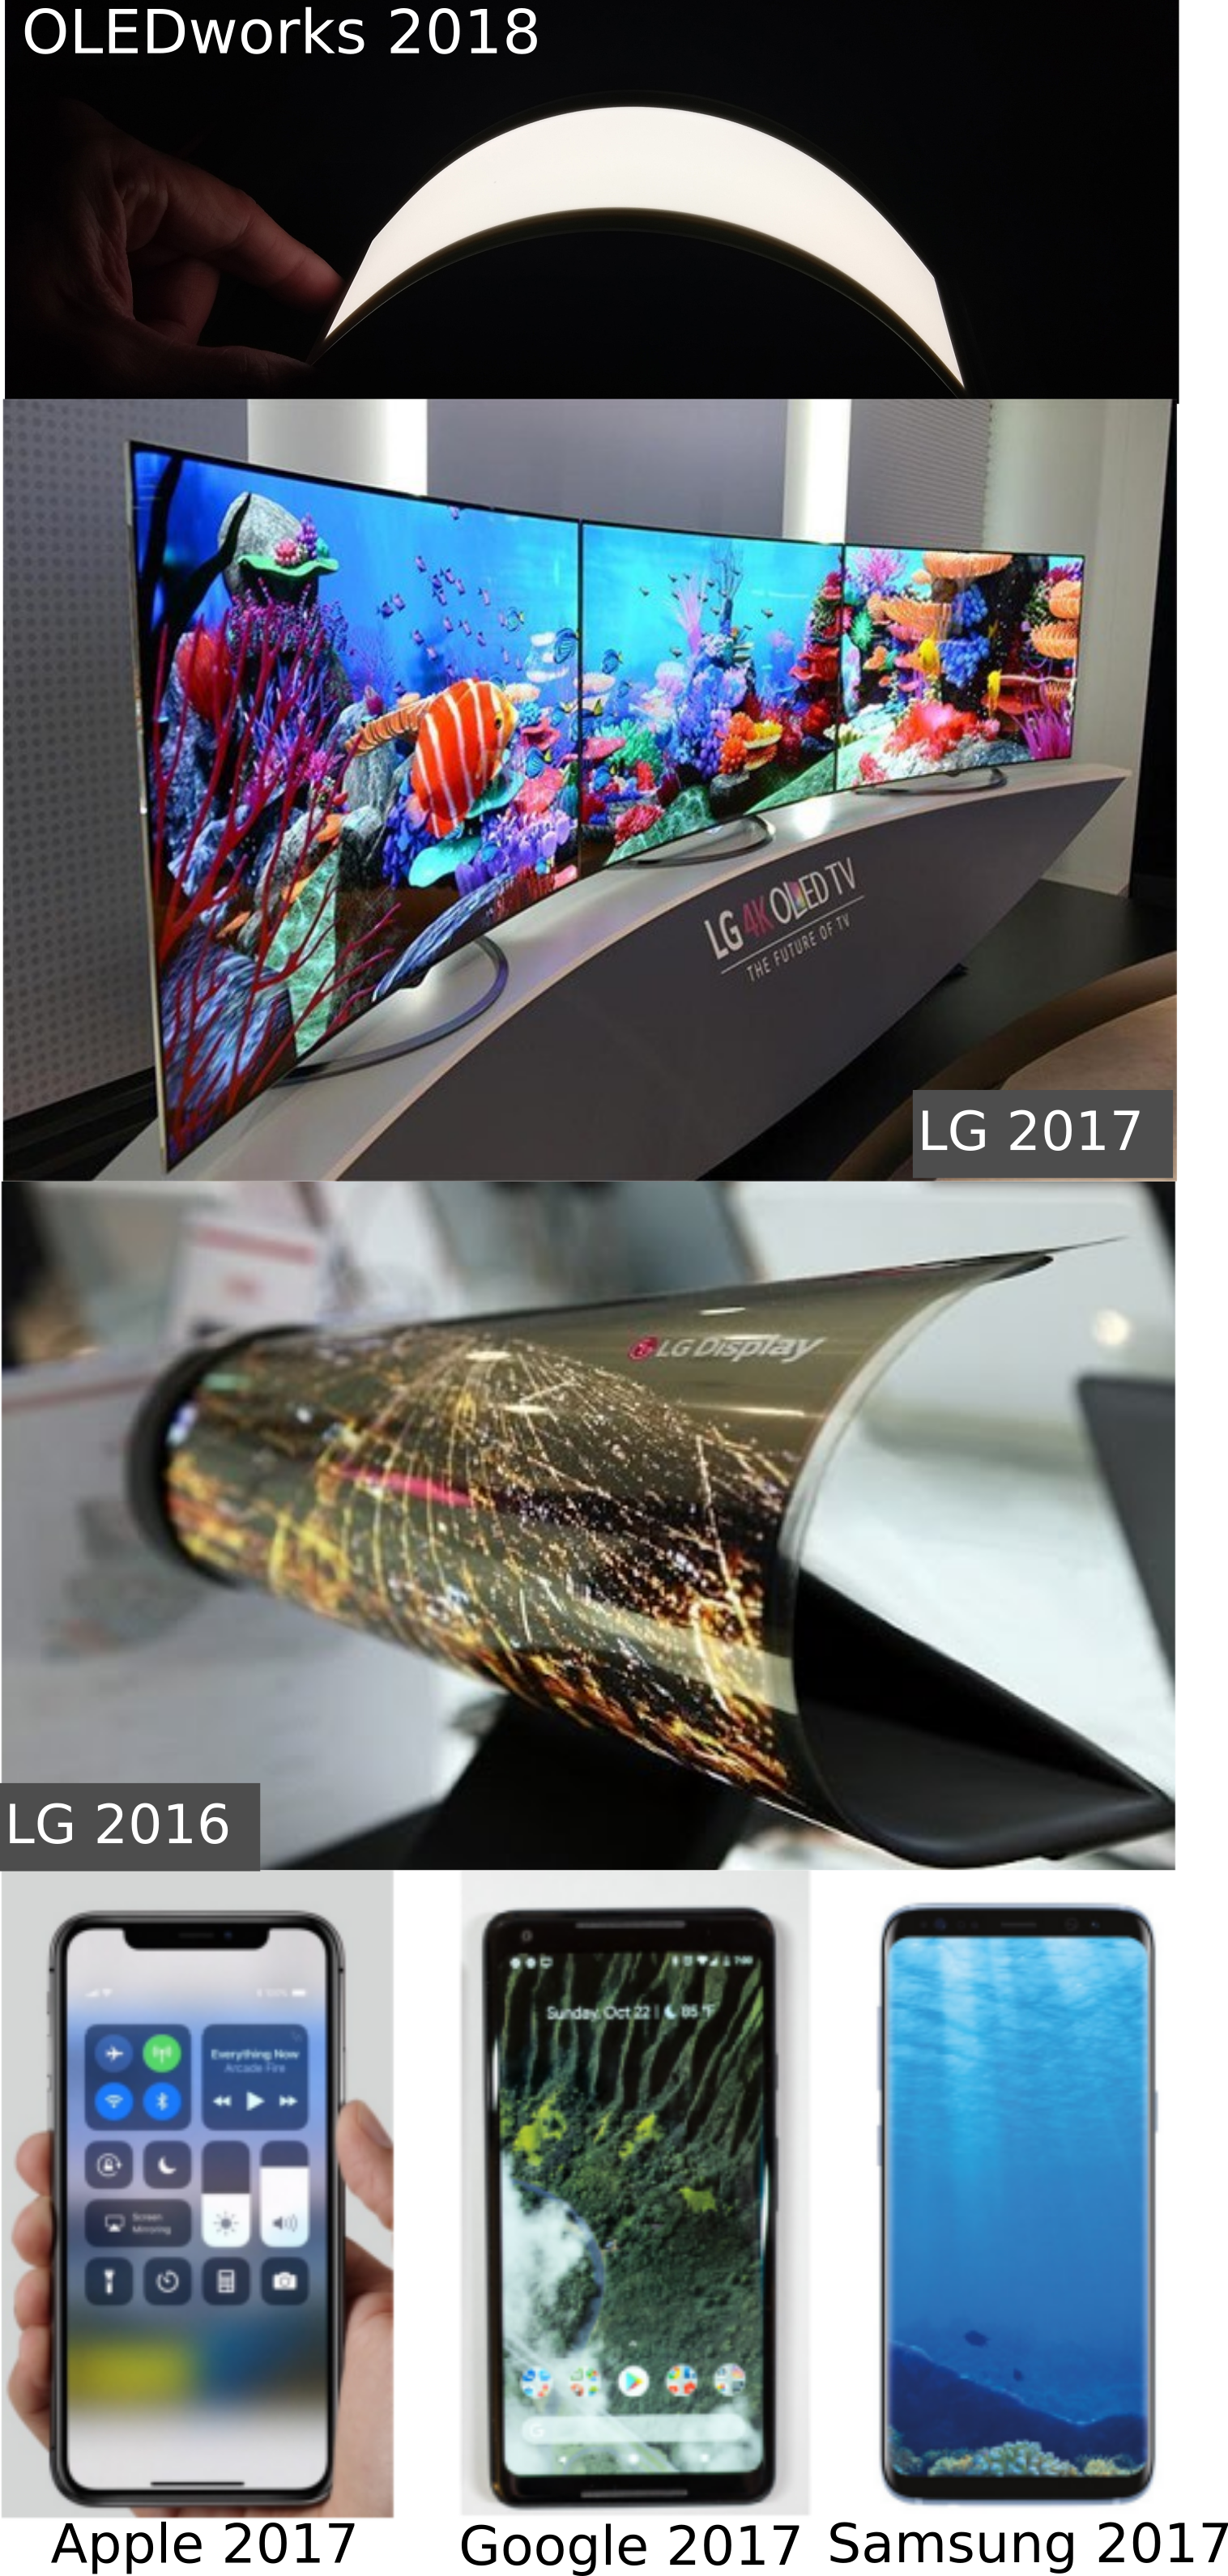
\includegraphics[width=.43\textwidth]{commercial/displays}
\caption{(Top) Commercial OLED white lighting from OLEDworks. (Middle) Flexible OLED TV demo from LG.  (Bottom) Smartphones from Apple, Google and Samsung.}
\label{fig:commercial_displays}
\end{wrapfigure}

OLEDs are becoming a highly commercialized technology and have had the most success of organic electronic applications.\supercite{Han2014a,Soneira2016,Soneira2017,Kalyani2017}
OLEDs offer improved contrast and viewing angle with similar power consumption when compared with LCD LED technology, which utilizes a white backlight in combination with color filtering layers to produce the image. \supercite{Morrison2017} 
These advantages in combination with the thin form factor and compatibility with curved and flexible substrates has made OLEDs excel in the small display market, including wearables and smartphones.
Flagship phones from all major manufacturer within the U.S. are utilizing OLEDs, including Samsung, Google, Apple and LG, and are shown in Figure \ref{fig:commercial_displays}.\supercite{Rozario2017,Morrison2018}
Several devices feature curved displays, offering a unique customer experience.

Large format displays are also commercially available for televisions.\supercite{Rozario2017,Morrison2018}
Again these displays advertise superior contrast and viewing angle.
A flexible large display is seen in Figure \ref{fig:commercial_displays}, demonstrated by LG, though not available for purchase.\supercite{Statt2016}
While large format displays offer significant advantage in viewer experience over LED technology, cost has prohibited commercialization.\supercite{Statt2016}
With a significant increase in cost compared to similar LCD LED devices, OLED TVs require a price reduction to see an improved market share above the current 1.1\%.\supercite{Statista2018}

Commercial white lighting is also available featuring OLED technology.
However, OLEDs suffer from significant drawbacks in this space, limiting the scope of their application.\supercite{Statt2016}
%With lower power efficiency than LEDs, the operational cost is higher, though not significantly.
%However, the power usage in combination with a 
OLED panels show shorter lifespan due to degradation (gradual luminance loss) as well as catastrophic failure (dark segment formation) making OLEDs significantly more expensive over their lifetime.
This could be reduced by device cost, but OLED fixtures are still more expensive than their LED counterparts.
Due to these drawbacks, OLEDs in white lighting are mostly used for architectural applications taking advantage of their thin form factor and flexibility.\supercite{OLEDWorks,Evangeline2018}
An example of this is shown in Figure \ref{fig:commercial_displays}, demonstrating both of these properties.\supercite{Statt2016}
OLED technology for white lighting could become competitive as the manufacturing technology and lifetime of devices improve.
Additionally, OLEDs currently suffer from a small market share, and cannot take advantage of the cost savings of large scale manufacturing.



\subsection{Organic Photovoltaics (OPVs)}

\begin{wrapfigure}{r}{.43\textwidth}
\centering
\includegraphics[width=.41\textwidth]{commercial/solar_cells}
\caption{a. Belectric solar cells. b. Transparent solar cell from Michigan State University.  c. Flexible solar cell from InfinityPV.}
\label{fig:commercial_solar}
\end{wrapfigure}

OPVs share all of the same form factor benefits of OLEDs.  
Because of this, OPVs are successful in a few novel implementations that are inaccessible for silicon panels.\supercite{Schlenker2011,Sapkota2014,Kenning2017,Gregg2003,Peumans2003}

Crystalline silicon solar cell panels suffer from their large and heavy form.
Due to their thin form factor, OPVs are a good option for areas where traditional panels cannot be installed.\supercite{FitzgeraldWeaver2017,Wesoff2014}
Figure \ref{fig:commercial_solar}a shows a canopy made of OPVs, utilizing an area inaccessible to traditional panels.
This is further extended by the ability to have flexible solar cells, shown in Figure \ref{fig:commercial_solar}b.\supercite{InfinityPV2018}


Due to the wide range of absorption bands available to OPVs, it is possible to form transparent solar cells.
Though these cells let through all visible light and thus suffer from low efficiency, they capitalize on areas where transparency is needed that could not facilitate opaque panels.
The transparent cells, shown in Figure \ref{fig:commercial_solar}c, are designed for window cells, where a traditional window can be replaced by a solar unit..\supercite{Henion2017,Cuthbertson2017}
This is extremely promising in urban environments and high rise buildings, where horizontal surfaces are at a premium, but windows are in abundance.


%However, they do not share the same high efficiency compared to their traditional counterparts. \supercite{NREL2018} 

\subsection{Organic Field-Effect Transistors (OFETs)}

Organic Field-effect transistors (OFETs) are an essential counterpart to the other devices we have discussed here.
On their own, OFETs can take advantage of their low cost and flexible form factor for use in cheap, low complexity electronics.  This can include Radio frequency ID (RFID) and single use medical devices.\supercite{Briseno2006a,Dimitrakopoulos2002,Sirringhaus2014,Yun2014,Briseno2006}
Additionally, OFETs are an essential part of OLED displays utilizing flexible behavior.

\section{Scope of This Thesis}

This thesis focuses on the understanding and improvement of OLEDs.
In particular, a fundamental understanding of the kinetic processes undergone during device operation is sought.
This kinetic understanding approach is desired to help in the optimization of device efficiency and lifetime through a better understanding and quantization of device behavior.
In addition to this kinetic understanding, lifetime is sought to be improved through the development of blue emitters, which are known to be limiting for device lifetime.



\ifcsdef{mainfile}{}{\printbibliography}
\end{document}
